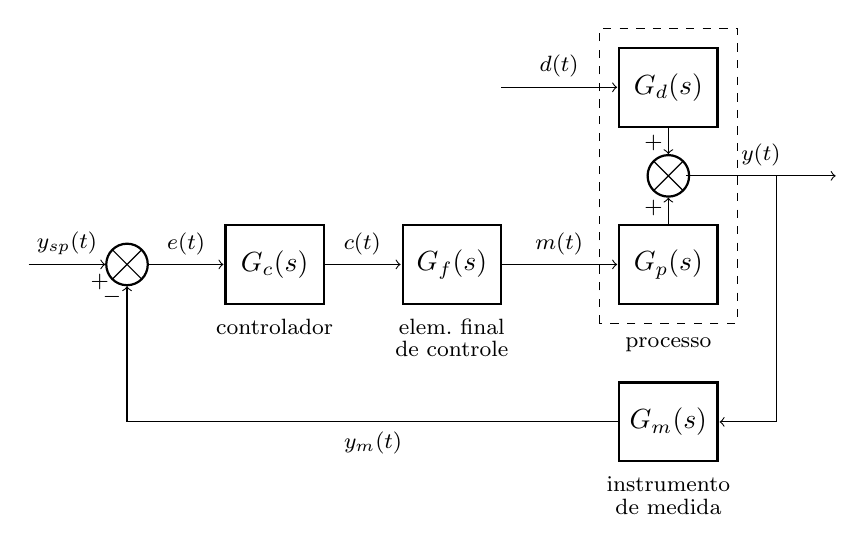
\begin{tikzpicture}[scale=5]
	\begin{scope}
	\draw [thick] (0,0) circle (1.5pt);
	\draw (-0.038,-0.038) node[below]{\footnotesize$-$} -- (0.038,0.038)  (0.038,-0.038)  -- (-0.038,0.038);
	\draw [->] (-0.25,0) -- node[above]{\footnotesize $ y_{sp}(t)$} (-0.055,0)node[below,xshift=-2]{\footnotesize$+$};
	\end{scope}
	\draw [->] (0.055,0) -- node[above]{\footnotesize $ e(t)$} (0.245,0);
	\draw [thick] (0.25,-0.1) rectangle node[]{$G_c(s)$} node[below=16]{\footnotesize controlador} (0.5,0.1);
	\draw [->] (0.5,0) -- node[above]{\footnotesize $ c(t)$} (0.695,0);
	\draw [thick] (0.7,-0.1) rectangle node[]{$G_f(s)$} node[below=16]{\footnotesize elem.\ final} node[below=24]{\footnotesize de controle} (0.95,0.1);
	\draw [->] (0.95,0) -- node[above]{\footnotesize $ m(t)$} (1.245,0);
	\draw [thick] (1.25,-0.1) rectangle node[]{$G_p(s)$} (1.5,0.1);
	\draw [->] (0.95,0.45) -- node[above]{\footnotesize $ d(t)$} (1.245,0.45);
	\draw [thick] (1.25,0.35) rectangle node[]{$G_d(s)$} (1.5,0.55);
	\draw [->] (1.42,0.225) -- node[above]{\footnotesize$ y(t)$} (1.8,0.225);
	%\draw [->] (1.375,0.3) -- (1.375,0.105);
	\draw [->] (1.375,0.35) -- (1.375,0.28);
	\draw [->] (1.375,0.1) -- (1.375,0.17);
	%\draw (1.375,0.225) circle [radius=1.2pt] node{+};
	\begin{scope}[shift={(1.375,0.225)}]
	\draw [thick] (0,0) circle (1.5pt);
	\draw (-0.038,-0.038) node[below]{\footnotesize$+$}  -- (0.038,0.038)  (0.038,-0.038)   -- (-0.038,0.038) node[above]{\footnotesize $+$};
	\end{scope}
	\draw [dashed] (1.2,-0.15) rectangle node[below=55] {\footnotesize processo} (1.55,0.6);
	\draw [thick] (1.25,-0.5) rectangle node[]{$G_m(s)$} node[below=16]{\footnotesize instrumento} node[below=24]{\footnotesize de medida} (1.5,-0.3);
	\draw [->] (1.65,0.225) -- (1.65,-0.4) -- (1.505,-0.4);
	\draw [->] (1.25,-0.4) -- node[below]{\footnotesize$ y_m(t)$} (0,-0.4) -- (0,-0.055);
\end{tikzpicture}